% Ikigai | Entry 08
\begin{ArtPage}
\EntryStart
\begin{center}
{\Fontgaramondbold\fontsize{6.5}{9}\selectfont\color{Muted}ENTRY 08\par}
\vspace{0.8cm}
{\Fontgaramond\fontsize{43}{50}\selectfont\color{Ink}Ikigai\par}
\vspace{0.15cm}
{\Fontcjk\fontsize{15}{19}\selectfont\color{Ink}生き甲斐\par}
\vspace{0.2cm}
{\Fontgaramond\fontsize{6.5}{9}\selectfont\color{Muted}%
  [ee-kee-gah-ee] \enspace·\enspace NOUN\par}
\vspace{0.8cm}
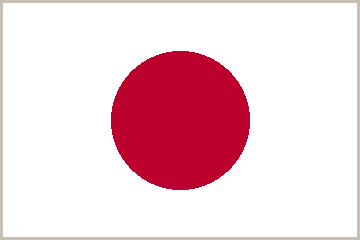
\includegraphics[height=.55cm,keepaspectratio]{assets/flags/flag_japan.png}\par
\vspace{0.2cm}
{\Fontgaramond\fontsize{6.5}{9}\selectfont\color{Muted}JAPANESE / JAPAN\par}
\end{center}
\EntryRuleBlock
\begin{minipage}{.92\linewidth}
\centering
{\Fontgaramond\fontsize{14}{18}\selectfont\color{Ink}%
  Something that makes life feel meaningful or worthwhile; a source of purpose,
  fulfillment, or a reason for living.\par}
\end{minipage}
\EntryDefinitionGap
\begin{center}
{\Fontgaramonditalic\fontsize{17.5}{22}\selectfont\color{Poetic}%
  “The little or great things that make tomorrow worth waking up for.”\par}
\end{center}
\EntryFooterGap
\begin{center}
{\Fontgaramond\fontsize{6}{8}\selectfont\color{Muted}THE ART OF PURPOSE\par}
\vspace{0.3cm}
{\Fontgaramond\fontsize{5.5}{7}\selectfont\color{Muted}%
  THE ART OF BEING \enspace·\enspace ENTRY 08\par}
\end{center}
\EntryBottomSpace
\end{ArtPage}

\begin{ArtFullPage}
\noindent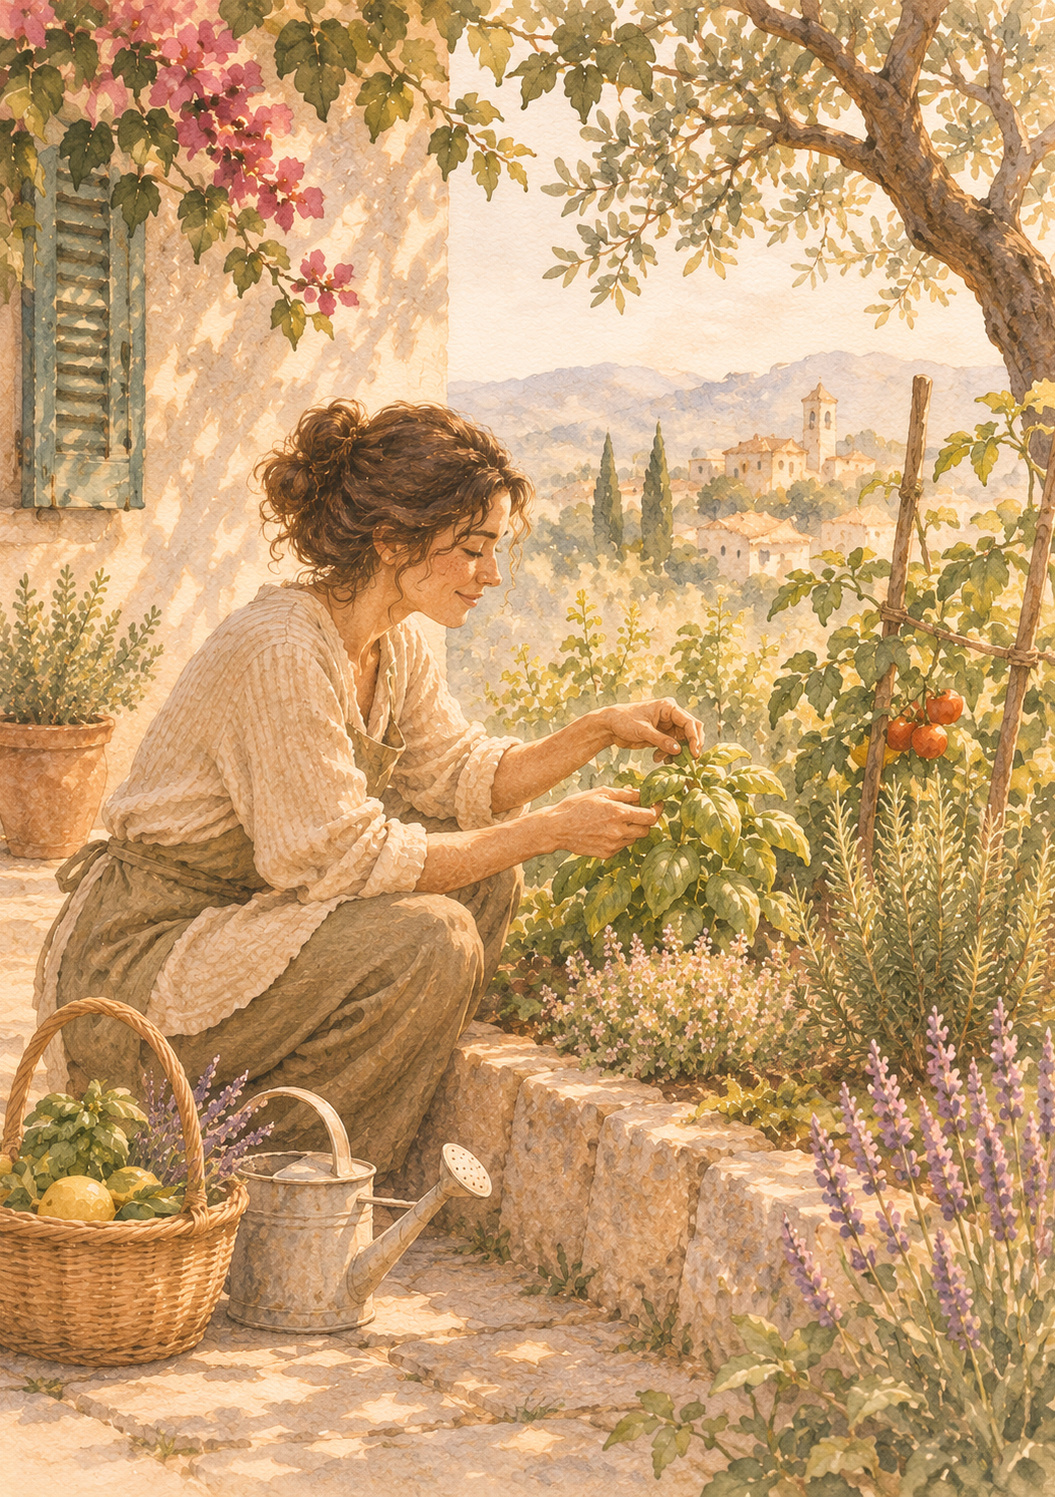
\includegraphics[width=\paperwidth,height=\paperheight]{assets/illustrations/08_ikigai.jpg}
\end{ArtFullPage}
